\chapter{Mediul Virtual}\label{MediulVirtual}
În acest capitol vom descrie mediul Unity în care se desfășoară simularea.
O scena în Unity este compusa dintr-o mulțime de \textbf{GameObjects}, care interacționează intre ele în timpul jocului, sau care prezintă doar aspecte estetice.
\begin{wrapfigure}{l}{0.25\textwidth} %this figure will be at the right
	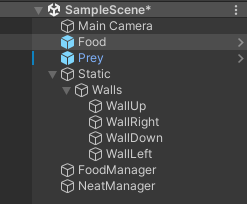
\includegraphics[width=0.25\textwidth]{images/scene_structure.png}
\end{wrapfigure}
Mai departe vom prezenta obiectele din cadrul simulării, proprietăților lor, și cum interacționează cu celelalte obiecte din mediu.
Structura scenei a fost inspirata din proiectul "Simulated Fish Ecosystem"\cite*{ZolphiteNeatYoutube}.

\section{Vizualizarea principala}
În mod implicit, înainte sa dam start oricărei simulări, în mediu avem 2 structuri principale: camera(\textbf{Main Camera}) și pereții(\textbf{Walls}).
\textbf{Main Camera} stabilește dimensiunea \textbf{Game view}-ului (poate fi văzut ca preview în coltul de dreapta jos a  imaginii \ref{fig:mainCameraView}, unde de-asemenea putem vedea cu o linie gri subțire marginea view-ului), cat și culoarea din background.
Pentru view-ul prezentat de camera nu avem o dimensiune standard, deoarece o schimbam depinzând de cantitatea de mâncare și de cate creaturi vrem sa folosim în cadrul unei simulări, însa păstram un aspect de imagine constant de 16:9.
Obiectul "Walls" este compus din 4 pereți(reprezentați ca segmente albe în cadrul imaginii \ref{fig:mainCameraView}): \textbf{WallUp}, \textbf{WallRight}, \textbf{WallDown} si \textbf{WallLeft}.
Aceștia sunt obiecte statice, care nu se mișca în timpul simulărilor.
Dimensiunea lor de asemenea nu este standard, dar la scalare menținem același aspect de imagine precum camera.
Fiecare dintre pereți are atașat un \textbf{Box Collider 2D} care este setat ca fiind Trigger, pentru a detecta coliziunile cu alte obiecte, și un \textbf{Rigidbody 2D} static plus tag-ul "Wall", pentru a putea fi detectați prin intermediul \textbf{Raycast}(detalii în secțiunea \ref{Senzori}).
Atunci când scalam pereții pentru diferite experimente o facem astfel încât marginile interioare ale pereților sa fie în afara marginilor view-ului camerei, deoarece la generarea cu coordonate aleatorii ale mâncării și ale creaturilor, acestea sunt generate intre marginile game view-ului, iar pereții fiind în afara lui evitam generarea obiectelor în pereți.

\begin{figure}[h]
	\centering
	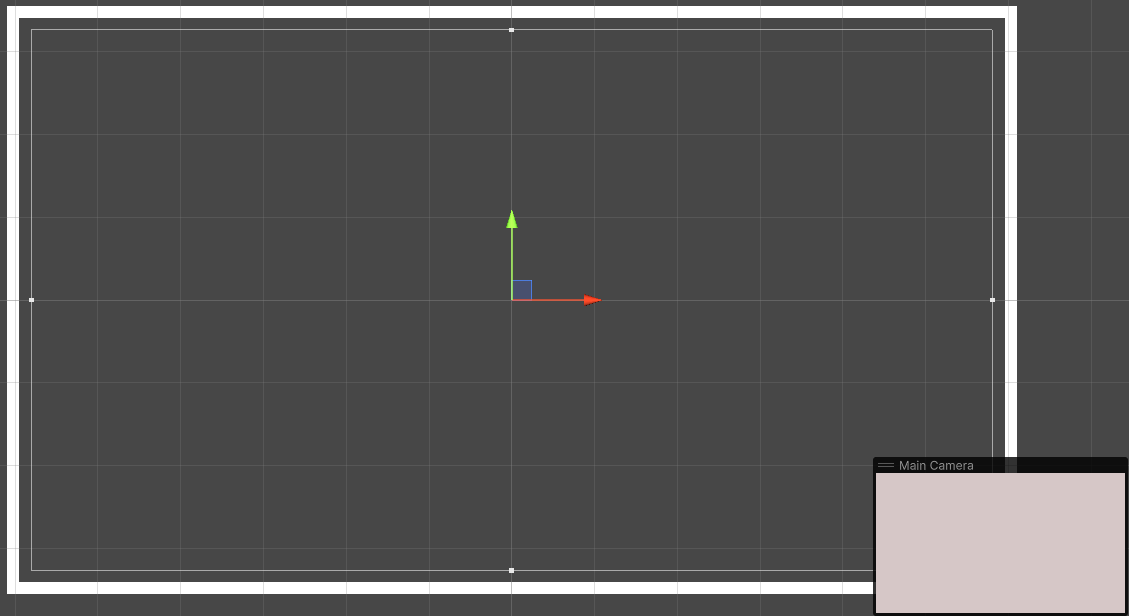
\includegraphics[width=0.75\textwidth]{images/unity_camera-view.png}
	\caption{Main camera view din Unity}
	\label{fig:mainCameraView}
\end{figure}

\section{Mâncarea}
Obiectele din ciclul de generare a mâncării sunt 2, \textbf{Food (Prefab asset)}(componente în imaginea \ref{fig:foodPrefab}) și \textbf{FoodManager}.
\textbf{Food Prefab} reprezinta schema după care se construiește o bucata de energie.
Bucățile de energie se găsesc pe harta sub forma de discuri de culoare galbena, mai exact \#F6F800.
Acestea, ca și pereții, reprezint obiecte statice care odată create nu se mișca.
\textbf{Food Prefab} are asociate următoarele componente:
\begin{itemize}
	\item \textbf{Circle Colider 2D} permite detectarea coliziunilor cu Obiectul
	\item \textbf{Rigidbody 2D} permite ca obiectul sa poată fi lovit de Raycasts
	\item \textbf{Food Controller} un script C\# care controlează distrugerea obiectului.
\end{itemize}
Obiectele construite prin FoodPrefab au scala de 1 pe axa X, Y și Z, și sunt asociate cu tag-ul "Food" pentru a permite detecția lor prin Raycasts și coliziuni.
De asemenea, ele sunt asociate cu \textbf{"Layer"}-ul "Food" pentru a permite detecția lor de către senzorul "Field of View"(secțiunea \ref{Senzori}).
\begin{figure}[h]
	\centering
	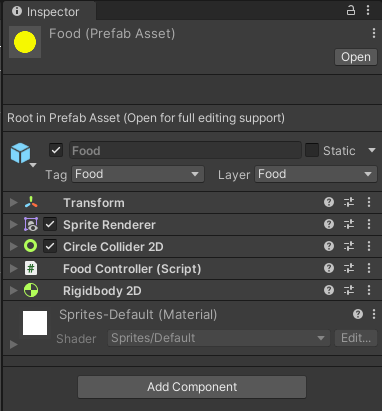
\includegraphics[width=0.5\textwidth]{images/food_prefab.png}
	\caption{Componentele Prefab-ului Food}
	\label{fig:foodPrefab}
\end{figure}

\textbf{FoodManager} este un "Empty Object", al cărui singur scop este sa fie un obiect permanent în aplicație de care putem atașa un script.
Scriptul pentru \textbf{FoodManager} ne permite sa asociem acestuia un "Prefab", în cazul acesta \textbf{Food Prefab}, iar scriptul ne oferă funcții pentru a crea un obiect sau mai multe din "Prefab-ul" asociat, și ne permite și sa le distrugem pe toate.
În \textbf{Food Controller}, scriptul pentru \textbf{FoodPrefab}, funcția "DieAndRespawn" permite distrugerea obiectului Food și regenerarea sa într-o alta locație în mediu, printr-un apel la FoodManger.
Astfel putem păstra numărul de bucăți de energie constant în mediu, chiar dacă energia este colectata în continuu de speciile de prada.

\section{Creaturile}
În mediul nostru virtual avem doua tipuri de creaturi, \textbf{Prada} si \textbf{Pradator}, care pot fi construite prin intermediul \textbf{Prey (Prefab Asset)} și respectiv \textbf{Predator (Prefab Asset)}.
În aceasta vom enunța în mare parte proprietățile pentru \textbf{Prey Prefab}, deoarece cele 2 prefaburi au multe elemente comune, deci pentru \textbf{Predator Prefab} vom expune doar diferențele.
\begin{figure}[h]
	\centering
	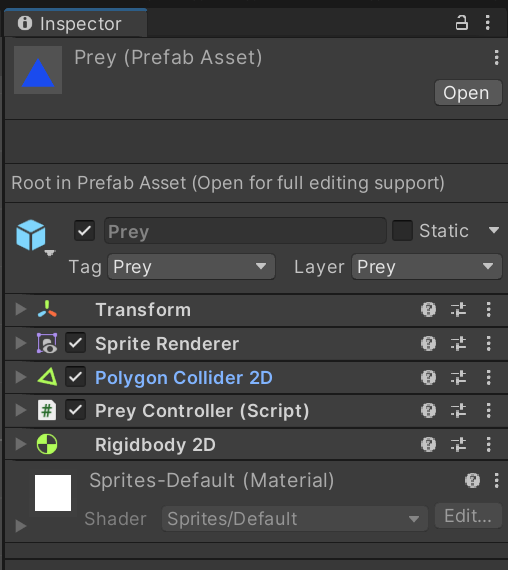
\includegraphics[width=0.5\textwidth]{images/prey_prefab.png}
	\caption{Componentele Prefab-ului Prey}
	\label{fig:preyPrefab}
\end{figure}

Prefab-ul pentru Prey definește următoarele componente:
\begin{itemize}
    \item \textbf{Sprite Renderer}: Definim forma creaturilor prey ca fiind un triunghi, scalat la dimensiunea de 1.5 pe axa x si Y
    \item \textbf{Polygon Collider 2D}: Un Collider care ia forma sprite-ului, folosit pentru detectarea coeziunilor
    \item \textbf{Rigidbody 2D}: Necesar pentru detectarea coliziunilor, pentru ca detectarea coeziunilor se va face în cadrul obiectelor dinamice: Prey si Predator. 
    Este de tip "Kinematic", spre deosebire de static pentru obiectele statice, și permite detectarea coeziunilor kineamtic/static și kinematic/kinematic.
    \item \textbf{Prey Controller}: script C\#, moștenește clasa \textbf{Creature Controller}, care încapsulează trăsături comune atât pentru prey cat și pentru predator, definește mișcarea, senzorii, acumularea de energie și moartea obiecte Prey.
\end{itemize}

\subsection*{Mișcarea}
Mișcarea este definita de schimbări care au loc asupra vitezei și a unghiului de rotație al creaturii. O creatura se poate deplasa doar în fata sau în spate, dar aplicând rotații asupra proprietății "transform.eulerAngles" se poate schimba direcția în care aceasta merge.
Schimbările asupra vitezei și a rotației obiectului sunt determinate de o rețea neuronala asociata obiectului, care primește ca input un număr de valori senzor, și returnează doua valori în intervalul (-1, 1), prima fiind modificarea asupra accelerației iar a doua modificarea asupra rotației.
Acest proces are loc în funcția "FixedUpdate()", deci la fiecare schimbare de frame stratul de intrare se încarcă cu valorile senzorilor, se executa pasul de feed-forward iar valorile din stratul de ieșire sunt folosite pentru a modifica poziția creaturii.

\subsection*{Senzori}\label{Senzori}
În mod implicit, toate creaturile au următorii senzori:
\begin{itemize}
    \item \textbf{Bias}: este un senzor care are mereu valoarea 1, folosit pentru a adăuga bias la nodurile care creează o conexiune cu el.
    \item \textbf{Perete}: acesta este un singur senzor, definit de un Raycast în fata obiectului(în planul 2D, aceasta reprezinta direcția "up" pentru proprietatea "transform" a obiectului). 
    Un raycast reprezinta proiectarea unei raze invizibile de o anumita lungime dintr-un punct, pe o direcție in scena.
    Când aceasta lovește collider-ul unui alt obiect din scena, este returnat un obiect din clasa "RaycastHit2D"(pentru mediul nostru 2D), care poate fi analizat pentru a determina ce tip de obiect a fost lovit(prin intermediul tag-ului) obiectului, și distanta de la punctul de pornire la care a fost lovit.
    Pentru senzorul de pereți, dacă raycast-ul lovește un perete, valoarea sa va fi raportul dintre distanta pana la lovitura și lungimea razei(deci, intre 0 și 1). Dacă nu a fost detectat un perete, valoarea senzorului e 1.  
    \item \textbf{Viteza curenta}: valoarea senzorului este valoarea precedenta a ieșirii pentru "viteza" a rețelei neuronale.
    \item \textbf{Unghi}: unghiul curent, exprimat intre -1 și 1, dintre direcția înainte a creaturii și axa $Y$ a scenei.
\end{itemize}
Pentru detecția țintelor creaturilor(adică a surselor de energie pentru fiecare tip în parte, prădătorii detectează creaturi de tipul prada, iar prada detectează bucățile de energie), am folosit în timp 2 tipuri de senzori.
Cel mai simplu reprezinta un sistem format din 3 Raycast-uri, o sa îl numim \textbf{fork} pentru a ne referi la el mai departe, care acționează la fel ca senzorul implicit pentru perete, doar ca în loc sa detecteze pereți, detectează țintele creaturii.
Un raycast este proiectat pe direcția înainte a obiectului, iar celelalte doua la un unghi de $45^{\circ}$ respectiv $-45^{\circ}$ fata de aceeași direcție.
\\
Ulterior am dezvoltat un senzor mai complex, de tip "Field of View", al cărui concept vine din \cite{rtNEAT}, secțiunea 5, figure 10, unde sunt descriși mai multi senzori printre care și "Enemy Radars".
Acesta descrie divizarea spațiului de $360^{\circ}$ din jurul agentului în mai multe zone. Fiecare zona activează un senzor în dependenta de cat de apropiat este un inamic de agent. Dacă sunt mai multi inamici în aceeași zona, se sumează activările pentru fiecare inamic în parte.
\begin{figure}[ht]
	\centering
	\animategraphics[autoplay,loop,width=\textwidth]{20}{images/sensors_showcase/sensors_showcase-}{9}{111}
	\caption{Senzorul FoV si senzorul pentru perete din cadrul prazii, liniile colorate arata distnata pana la fragmentele de energie care sunt detectate de diferitele zone ale senzorului. Linia alba atunci cand prada se apropie de perete este raycast-ul catre perete}
    \label{fig:senzorDemo}
\end{figure}

În cadrul implementării noastre, pentru senzorul "Field of View"(\textbf{FoV}), alegem un unghi, intre 0 și 180 de grade, care reprezinta câmpul vizual din fata unei creaturi, și raza pana la care acesta se extinde.
Prin alt parametru, specificam în cate zone se împarte acesta. 
Prin intermediul metodei "Physics2D.OverlapCircleAll", se detectează toate țintele din cadrul unui cerc din jurul creaturii, după care, analizând unghiul dintre direcția înainte a creaturii și poziția unei ținte, putem determina dacă țintele cad în cadrul câmpului vizual, și în ce zona a câmpului.
Pentru fiecare zona, activarea ei va reprezenta valoarea calculului $\sum_{i} 1 - d_i/r$, $i$ fiind o ținta din cadrul zonei, $d_i$ distanta pana la ținta, iar $r$ raza cercului în care are loc detecția. Deci pentru fiecare ținta avem o activarea intre 0 și 1, care este mai mare cu cat ținta e mai aproape de creatura.
În cadrul animației \ref{fig:senzorDemo}, se poate vedea cum funcționează senzorul "FoW", cu un câmp vizual de $90^{\circ}$, împărțit în 3 zone, pe o distanta de 20 "world units", iar la sfârșitul animație putem vedea și o vizualizare a raycast-ului pentru senzorul de perete.
Pentru a scrie vizualizarea în "Editor View" a senzorului "FoW" un mare ajutor a fost \cite{FoWVisualization}.
În unul din experimentele de la capitolul \ref{Rezultate}, vom arata ca prada care folosește senzorul "FoW" este superioara celei care folosește "Fork", și vom prezenta și diferențele de comportament intre cele 2 tipuri de prada.
Pentru prădătorii la senzori nu se schimba nimic decât țintele căutate, acestea fiind creaturile de prada.

\subsection*{Coliziuni}
Datorita faptului ca toate obiectele care interacționează în cadrul scenei au asociat cate un collider și un rigidbody, putem detecta coliziunile intre ele.
Procesare acestor coliziuni se face în cadrul script-uri-lor "Prey Controller" și "Predator Controller", asociate prefab-ului "Prey" și respectiv "Predator".
Prin intermediul tag-urilor "Wall" și "Food", script-ul "Prey Controller" înregistrează coliziunile cu pereții, ceea ce cauzează moartea prăzii, și coliziunea cu fragmentele de energie, prin care energia asociata fragmentului este absorbita, iar fragmentul prin funcția "DieAndRespawn" este regenerat la alte coordonate aleatorii în cadrul scenei, deci cantitatea de energie în scena este constanta.
Procesare coliziunilor prada-prădător are loc în script-ul "Predator Controller", și pot fi identificate prin tag-ul asociat creaturilor de prada, "Prey". În cadrul acestor coliziuni, obiectul prada este distrus, însa obiectul prădător primește energie, într-o cantitate semnificativ mai mare decât ce primesc creaturile prada la coliziunile prada-fragment de energie, plus un procent din energia acumulata de prada de-a lungul vieții.
Facem aceste ajustări deoarece vânatul pentru prada este mult mai ușor decât cel pentru prădător,pentru ca prădătorii trebuie sa dezvolte comportamente de chassing, astfel ca prădătorii ar trebui sa primească mai multa energie din vânat pentru a ne asigura ca aceștia nu sunt surclasați de prada în cadrul evoluției.
Coeziunile prădător-perete sunt la fel ca la prada, însa prădătorii nu înregistrează coliziunile cu fragmentele de energie, deoarece vrem ca aceștia sa obțină energie doar prin coliziunile cu prada.
Pe tot parcursul vieții lor, creaturile consuma energie în mod constant, plus o cantitate care depinde de viteza cu care se mișca. Astfel le încurajam sa acumuleze energie încontinuu.
Odată ce o creatura rămâne fără energie, aceasta moare.

\section{Managementul Algoritmului}
\textbf{NeatManager}, ca și FoodManger, este un "Empty Object" pe care îl folosim pentru a atașa script-ul "Neat Manager".
Acest script este responsabil de desfășurare algoritmului Neat, deci are ca responsabilități generarea populației inițiale, înregistrarea morților, crearea generațiilor următoare și înregistrarea de log-uri despre populație pe parcursul generațiilor.
În cadrul NeatManager putem decide sa efectuam experimente în care folosim doar creaturile de prada, sau și prădătorii, și putem determina parametri cum ar fi numărul de membri, numărul de noduri pentru stratul de intrare cat și cel de ieșire etc.(vom discuta mai pe larg mulțimea de parametri în secțiunea \ref{SetariExperimentale}). 
Faza de generare a populației inițiale se desfășoară în următorul mod:
\begin{enumerate}
    \item Se generează genomul inițial pentru fiecare membru din populație(reprezinta o codificare Neat a unei rețele cu structura minima dar cu ponderi ale conexiunilor aleatorii, revedeți secțiunea \ref{InitializareNeat})
    \item Se generează fenotipul pentru fiecare genotip(rețeaua neuronala propriu-zisa, vom expune maparea de la fenotip la genotip în capitolul \ref{DetaliiImplementare})
    \item Se creează agenții simulării, După prefab-ul care a fost asignat către NeatManager. Proprietățile acestora sunt setate După parametrii NeatManager pentru un prefab specific, și sunt poziționați la coordonate aleatorii în cadrul "Main Camera View", fiecăruia dintre ei fiindu-i asignata și una dintre rețele create la pasul precedent.
\end{enumerate}
După creare, agenții sunt liberi sa exploreze mediul și sa acumuleze fitness. În secțiunea anterioara nu am menționat ca în toate scenariile în care un agent moare, asta fiind valabil atât pentru prada cat și pentru prădători, acesta își înregistrează moartea și cauza ei la "NeatManager", prin intermediul funcției "RegisterDeath".
Astfel, NeatManager poate determina când toți agenții din mediu au fost distruși, și poate începe crearea următoarei generații.
Înainte de crearea următoarei generații, se log-eaza fitness-ul average și fitness-ul celui mai bun agent din generația curenta, plus informații despre structura celui mai bun agent.
Procesul de generare a următoarei generații decurge la fel ca cel de inițializare, doar ca mai întâi se aplica o filtrare pentru a rămâne doar genom-urile cele mai bune din cadrul fiecărei specii, care vor trece prin procesul de crossover și de mutație pentru generarea genomurilor generației viitoare.
Aceste genom-uri sunt asignate către diferite specii din populație, care grupează genomuri similare. După acest pas se creează noile rețele neuronale, și se generează noii agenți care gândesc prin intermediul  acestora, iar tot procesul se repeta din nou la fiecare generație.
Ne-am permis în aceasta secțiune sa facem un rezumat al funcționarii algoritmului, vorbind despre obiectul care este responsabil de desfășurarea lui, însa în capitolul \ref{DetaliiImplementare} vom expune detaliat, cu exemple din cod, procesele din cadrul algoritmului.
